\chapter{Camera-Based Driver Monitoring} \label{cap:conceitos}

%\begin{itemize}
%    \item Definir as seções representativas em função do trabalho.
%    \item Apresentar os conceitos empregados e a revisão da literatura.
%    \item Citar os trabalhos consultados no texto.
%\end{itemize}

In this chapter, we introduce some interesting concepts analysed by the group when studying literature for camera-based driver monitoring systems.

\section{Near-Infrared (NIR) Imaging}

One of the primary challenges faced in the camera-based approach is maintaining consistent performance under varying lighting conditions, such as driving at night or through tunnels. According to \cite{review}, Near-Infrared (NIR) imaging is the standard solution to this problem. Unlike standard RGB cameras, NIR systems operating in the $850--940$ nanometer can capture facial features in total darkness. In our AIware project, if using an infrared camera is not possible, we can try to incorporate microphone-based based to help our model make good predictions even when image quality is suboptimal.

\section{Behavioral Biometrics: EAR and MAR Metrics}

To objectively quantify driver states like drowsiness and distraction, two of the most critical metrics are the Eye Aspect Ratio (EAR) and the Mouth Aspect Ratio (MAR).
\begin{itemize}
    \item \textbf{EAR} monitors the distance between eyelids to detect blinks and prolonged eye closure (micro-sleeps).
    \item \textbf{MAR} measures mouth opening levels to identify frequent yawning, a primary indicator of early-stage fatigue.
\end{itemize}

\begin{figure}[h!]
    \centering
    \caption{Eye Aspect Ratio metric \cite{bellino2018}}
    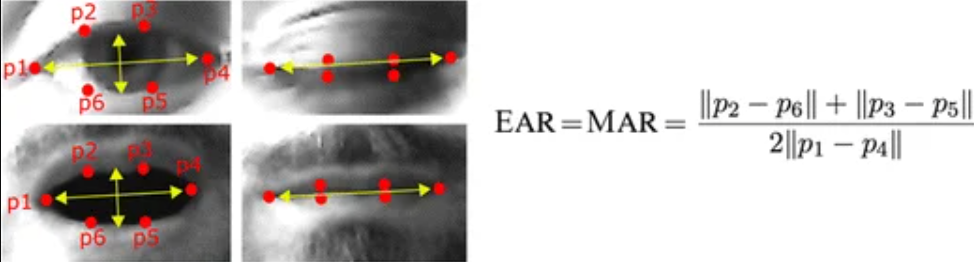
\includegraphics[width=.7\textwidth]{images/EAR.png}
    \label{fig:ear}
\end{figure}

\begin{figure}[h!]
    \centering
    \caption{Mouth Aspect Ratio metric \cite{zhu2022}}
    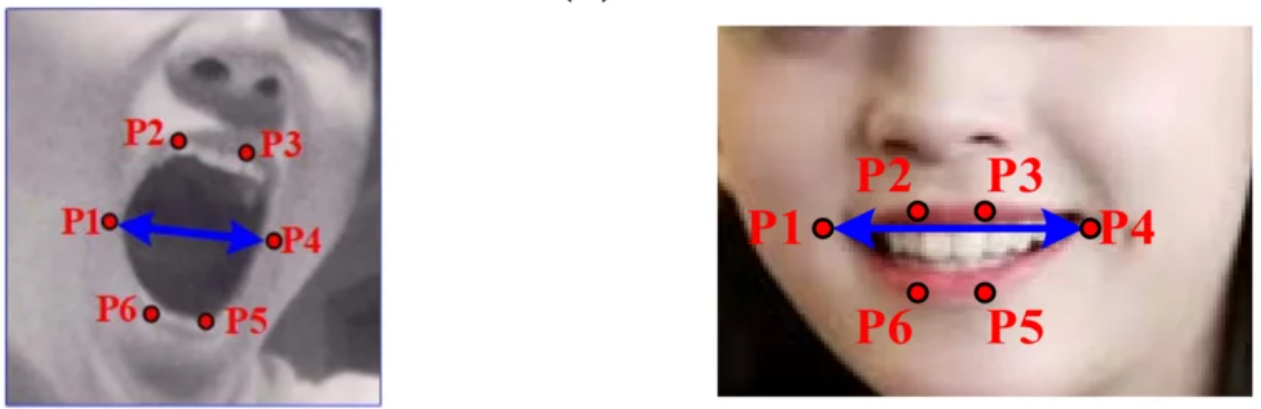
\includegraphics[width=.7\textwidth]{images/MAR.png}
    \label{fig:mar}
\end{figure}


According to \cite{review}, these geometric ratios allow lightweight AI models to perform binary classifications with high precision and low computational overhead, fitting the constraints of edge devices.

\section{Remote Photoplethysmography (rPPG)}

A more advanced concept discussed in recent literature is remote Photoplethysmography (rPPG), which allows for the detection of physiological signals such as heart rate and respiration using only a standard camera sensor. By analyzing minute skin color variations caused by blood circulation (which are often imperceptible to the human eye), the system can infer the driver's stress levels or sudden health emergencies. This is a very interesting technique, however it is unlike we will explore it for the AIware project in the Embedded Systems Laboratory course.